% 2006 四川理科 19：长方体 ABCD-A_1B_1C_1D_1 及题设中点、构造线
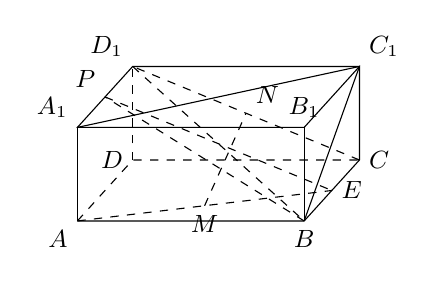
\begin{tikzpicture}[scale=0.9, font=\small]
  % 斜投影：AB=2a，AD=AA_1=a；比例仅用于示意。
  \coordinate (A)  at (0,0);
  \coordinate (B)  at (3.2,0);
  \coordinate (D)  at (0.78,0.86);
  \coordinate (C)  at (3.98,0.86);
  \coordinate (A1) at (0,1.32);
  \coordinate (B1) at (3.2,1.32);
  \coordinate (D1) at (0.78,2.18);
  \coordinate (C1) at (3.98,2.18);
  \coordinate (E)  at (3.59,0.43);
  \coordinate (P)  at (0.39,1.75);
  \coordinate (M)  at (1.795,0.215);
  \coordinate (N)  at (2.38,1.52);

  % 实线棱：前面、右侧及上部可见轮廓。
  \draw (A)--(B)--(C)--(C1)--(B1)--(A1)--(D1)--(C1);
  \draw (A)--(A1);
  \draw (B)--(B1);
  % 题图中的辅助线。
  \draw (A1)--(C1);
  \draw (B)--(C1);

  % 被遮挡的棱与位于后方/底面的构造线。
  \draw[dashed] (A)--(D)--(C);
  \draw[dashed] (D)--(D1);
  \draw[dashed] (A)--(E);
  \draw[dashed] (M)--(N);
  \draw[dashed] (P)--(E);
  \draw[dashed] (B)--(P);
  \draw[dashed] (D1)--(B);
  \draw[dashed] (C)--(D1);

  \node[below left] at (A) {$A$};
  \node[below] at (B) {$B$};
  \node[right] at (C) {$C$};
  \node[left] at (D) {$D$};
  \node[above left] at (A1) {$A_1$};
  \node[above] at (B1) {$B_1$};
  \node[above right] at (C1) {$C_1$};
  \node[above left] at (D1) {$D_1$};
  \node[above left] at (P) {$P$};
  \node[above right] at (N) {$N$};
  \node[below] at (M) {$M$};
  \node[right] at (E) {$E$};
\end{tikzpicture}
